\documentclass{article}
\usepackage[utf8]{inputenc}
\usepackage[spanish.mexico]{babel}
\usepackage[american voltages, american currents,siunitx]{circuitikz}
\usepackage{natbib}

%para fotos

\usepackage{graphicx}
\usepackage{subcaption}

\title{Previo 4}
\author{Pablo Vivar Colina\\
Grupo 13\\
}
%\date{Septiembre 2017}



\begin{document}

\maketitle

\section{Curvas de Lissajous}

En matemáticas, la curva de Lissajous, también conocida como figura de Lissajous o curva de Bowditch, es la gráfica del sistema de ecuaciones paramétricas correspondiente a la superposición de dos movimientos armónicos simples en direcciones perpendiculares:\citep{CurvasLiss}

\begin{equation}
    x = A sin ⁡ (ω x t + \alpha ) , y = B sin ⁡ ( ω y t + β ) , δ = \alpha  − β 
\end{equation}

    

Esta familia de curvas fue investigada por Nathaniel Bowditch en 1815 y después, con mayores detalles, por Jules Antoine Lissajous.\citep{CurvasLiss}\\

En mecánica clásica, la trayectoria de un movimiento armónico complejo bidimensional es una curva de Lissajous.\citep{CurvasLiss}

\begin{figure}[ht!]
    \centering
    \begin{subfigure}[b]{0.3\textwidth}
        \includegraphics[width=\textwidth]{Imagenes/Lissajous_curve_1by2.png}
        \caption{a=1,b=2}
        \label{fig:a1b2}
    \end{subfigure}
    ~ %add desired spacing between images, e. g. ~, \quad, \qquad, \hfill etc. 
      %(or a blank line to force the subfigure onto a new line)
    \begin{subfigure}[b]{0.3\textwidth}
        \includegraphics[width=\textwidth]{Imagenes/Lissajous_curve_3by2.png}
        \caption{a=3,b=2}
        \label{fig:a3b2}
    \end{subfigure}
    ~ %add desired spacing between images, e. g. ~, \quad, \qquad, \hfill etc. 
    %(or a blank line to force the subfigure onto a new line)
    \begin{subfigure}[b]{0.3\textwidth}
        \includegraphics[width=\textwidth]{Imagenes/600px-Lissajous_curve_3by4.png}
        \caption{a=3,b=4}
        \label{fig:a3b4}
    \end{subfigure}
    
    \\
    
    \begin{subfigure}[b]{0.3\textwidth}
        \includegraphics[width=\textwidth]{Imagenes/600px-Lissajous_curve_5by4.png}
        \caption{a=1,b=2}
        \label{fig:a1b2}
    \end{subfigure}
    ~ %add desired spacing between images, e. g. ~, \quad, \qquad, \hfill etc. 
      %(or a blank line to force the subfigure onto a new line)
    \begin{subfigure}[b]{0.3\textwidth}
        \includegraphics[width=\textwidth]{Imagenes/600px-Lissajous_curve_5by6.png}
        \caption{a=5,b=6}
        \label{fig:a5b4}
    \end{subfigure}
    ~ %add desired spacing between images, e. g. ~, \quad, \qquad, \hfill etc. 
    %(or a blank line to force the subfigure onto a new line)
    \begin{subfigure}[b]{0.3\textwidth}
        \includegraphics[width=\textwidth]{Imagenes/600px-Lissajous_curve_9by8.png}
        \caption{a=9,b=8}
        \label{fig:a9b8}
    \end{subfigure}
    
    
    \caption{Curvas Lissajous\citep{CurvasLiss}}\label{fig:Lissajous}
\end{figure}


\section{Frecuencia}

Frecuencia una magnitud que mide el número de repeticiones por unidad de tiempo de cualquier fenómeno o suceso periódico.\citep{Frec}\\

Para calcular la frecuencia de un suceso, se contabilizan un número de ocurrencias de éste, teniendo en cuenta un intervalo temporal, y luego estas repeticiones se dividen por el tiempo transcurrido. Según el Sistema Internacional (SI), la frecuencia se mide en hercios (Hz), en honor a Heinrich Rudolf Hertz. Un hercio es la frecuencia de un suceso o fenómeno repetido por segundo. Así, un fenómeno con una frecuencia de dos hercios se repite dos veces por segundo. Esta unidad se llamó originalmente «ciclo por segundo» (cps).
Otras unidades para indicar frecuencias son revoluciones por minuto (rpm o r/min según la notación del SI); las pulsaciones del corazón se miden en latidos por minuto (lat/min) y el tempo musical se mide en «pulsos por minuto» (bpm, del inglés “beats per minute”).\citep{Frec}\\


\begin{equation}
      1 H z = 1 s
\end{equation}
   

Un método alternativo para calcular la frecuencia es medir el tiempo entre dos repeticiones (periodo) y luego calcular la frecuencia (f) recíproca de esta manera:\citep{Frec}

\begin{equation}
     f = n T 
\end{equation}

   
donde T es el periodo de la señal.\citep{Frec}

\section{Ángluo de defasamiento}

En el caso de dos ondas sinusoidales, de igual pulsación $\omega$ , representadas matemáticamente como:

    $y 1 = A 1 cos ⁡ ( ω t − k x 1 + φ 1 ) $

y

    $y 2 = A 2 cos ⁡ ( ω t − k x 2 + φ 2 ) $,

el desfase Δ φ  en el instante t es:
\begin{equation}
   Δ φ = ( ω t − k x 2 + φ 2 ) − ( ω t − k x 1 + φ 1 )    
\end{equation}
   

Se comprueba que si las dos ondas tienen la misma frecuencia y que las posiciones no cambian, el desfase queda constante.\citep{Defase}\\

En cambio, si las frecuencias no son iguales, el desfase cambia con el tiempo. Ese caso se produce en los batimientos.\citep{Defase}\\

Si $\Delta \phi$  es positivo, la onda 2 está en avance con respecto a la onda 1. Y si $\Delta \phi$  es negativo, la onda 2 está en retardo con respecto a la onda 1.

\subsection{Oscilación Senoidal}

Una señal senoidal o sinusoidal, $a(t)$, tensión, $v(t)$, o corriente, $i(t)$, se puede expresar matemáticamente según sus parámetros característicos (figura \ref{fig:ondaSenoidal}), como una función del tiempo por medio de la siguiente ecuación:\citep{CA}

\begin{equation}
    a(t)=A_0 \cdot \sin(\omega t + \beta)
\end{equation}
\begin{itemize}
    \item $A_0$ es la ''amplitud'' en [V] o [A] (también llamado ''valor máximo o de pico'')
    
    \item $\omega$  pulsación en radianes/segundo
    
    \item $t$ el tiempo en [s]
    
    \item $\beta$ el ángulo de fase inicial en radianes.
\end{itemize}


Dado que la velocidad angular es más interesante para matemáticos que para ingenieros, la fórmula anterior se suele expresar como:\citep{CA}\\

\begin{equation}
    a(t)=A_0 \cdot \sin(2 \pi f t + \beta)
\end{equation}


donde ''f'' es la frecuencia (Hz) y equivale a la inversa del período $f=\frac{1}{T}$. Los valores más empleados en la distribución son 50 Hz y 60 Hz.\citep{CA}


\begin{figure}[ht!]
    \centering
    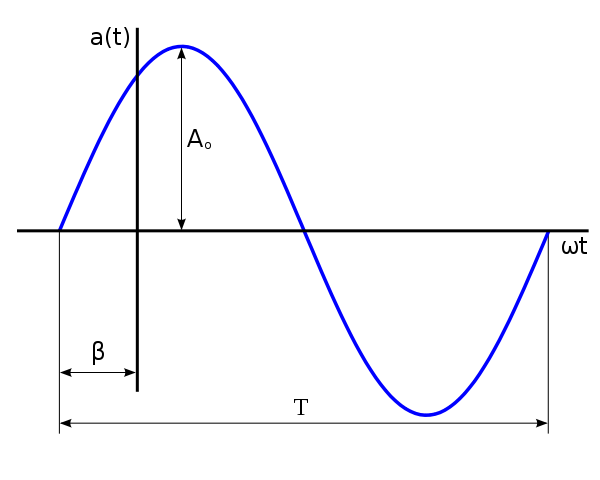
\includegraphics[scale=0.5]{Imagenes/600px-OndaSenoidal.png}
    \caption{Parámetros característicos de una oscilación sinusoidal.}
    \label{fig:ondaSenoidal}
\end{figure}


\bibliographystyle{plain}
\bibliography{Referencias.bib}


\end{document}